\chapter{Introduction}
\label{sec:introduction}

The availability of open source repositories like GitHub is driving
data-driven solutions to software engineering problems, e.g.
specification inference by ~\cite{nguyen2014mining}, discovering programming
patterns by ~\cite{thummalapenta2009alattin}, suggesting bug
fixes by ~\cite{livshits2005dynamine,cpminer}, etc.
These software engineering tasks analyze different source code
representations, such as text, abstract syntax trees (ASTs), control
flow graphs (CFGs), at massive scale.
The performance of source code analysis over graphs heavily depends on
the order of the nodes visited during the traversals: {\em the
traversal strategy}. While graph traversal is a well-studied problem,
and various traversal strategies exists; e.g., depth-first,
post-order, reverse post-order, etc, no single strategy works best for
different kinds of analyses and different kinds of graphs.
Our contribution is {\em hybrid traversal selection}, a
novel source code analysis optimization technique for source code
analyses expressed as graph traversals. This work was done collaboratively with Dr. Hridesh Rajan, Dr.Hoan A Nguyen and Ganesha Upadhaya. Consequently, Chapters 1, 2, 4 and 6 - 14 in this thesis are based on that collaborative work.

\begin{figure*}[t]%
\centering
\subfloat[Reaching definition analysis.] {
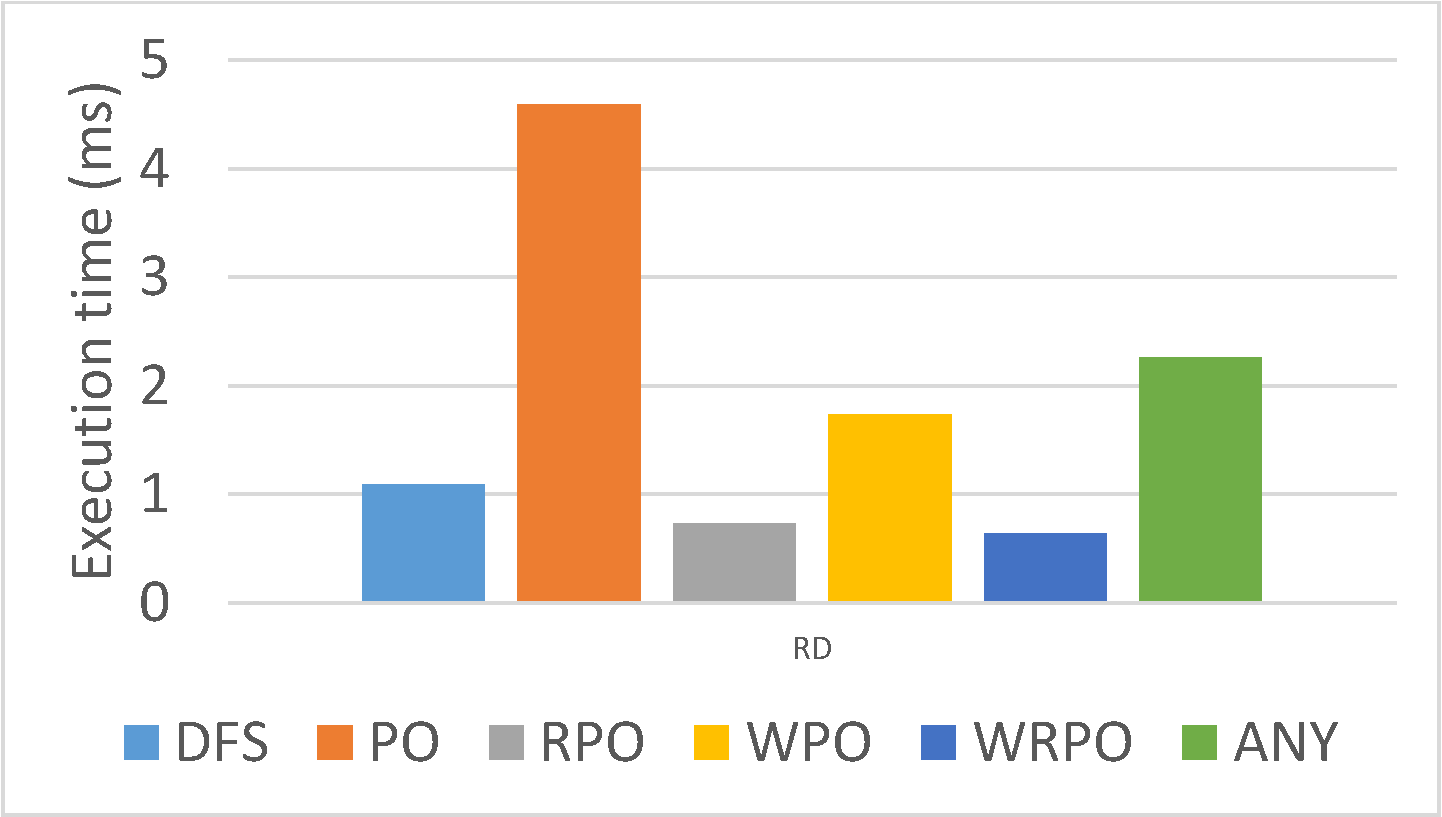
\includegraphics[width=.5\linewidth]{figures/motivation-a-rd}
}
\subfloat[Post-dominator analysis.] {
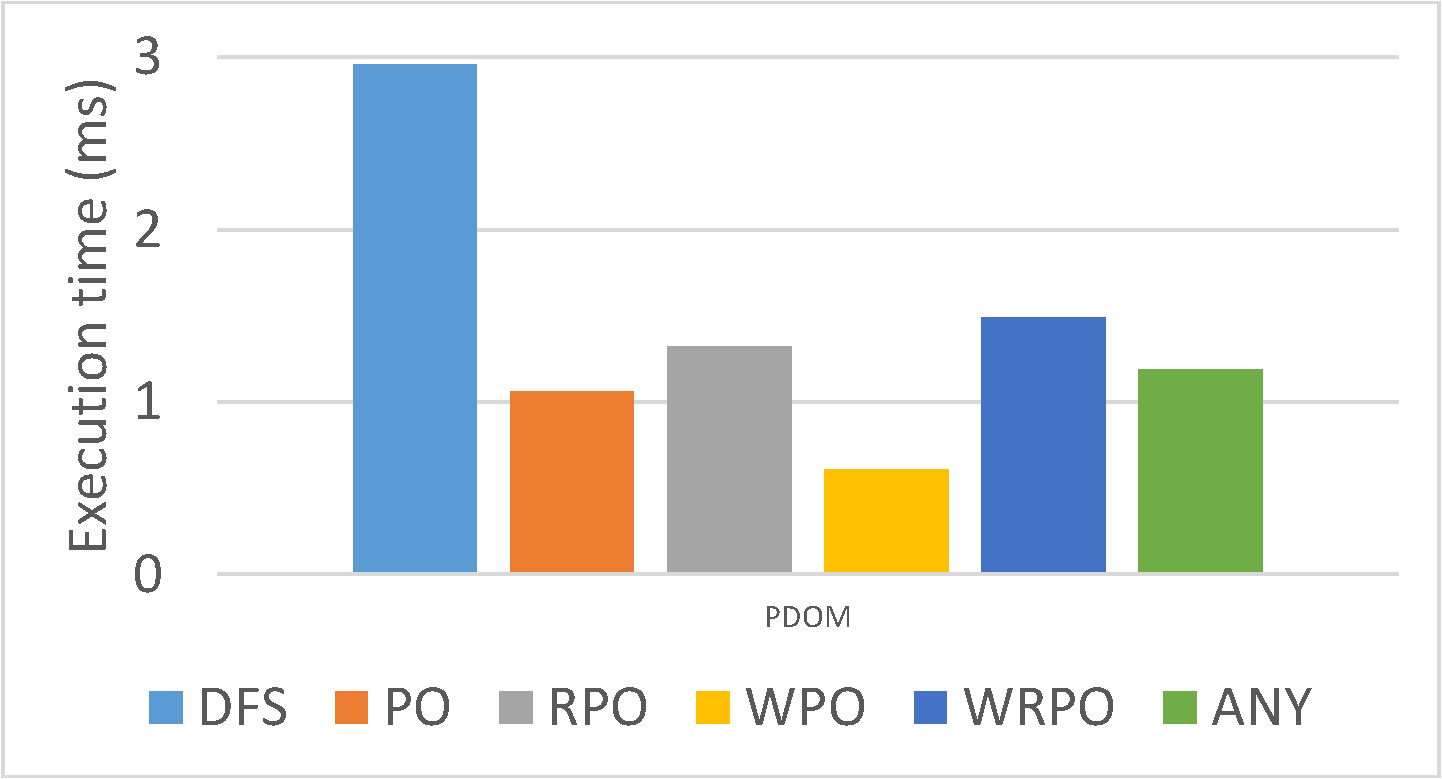
\includegraphics[width=.5\linewidth]{figures/motivation-a-pdom}
}\\
\subfloat[Collector analysis.] {
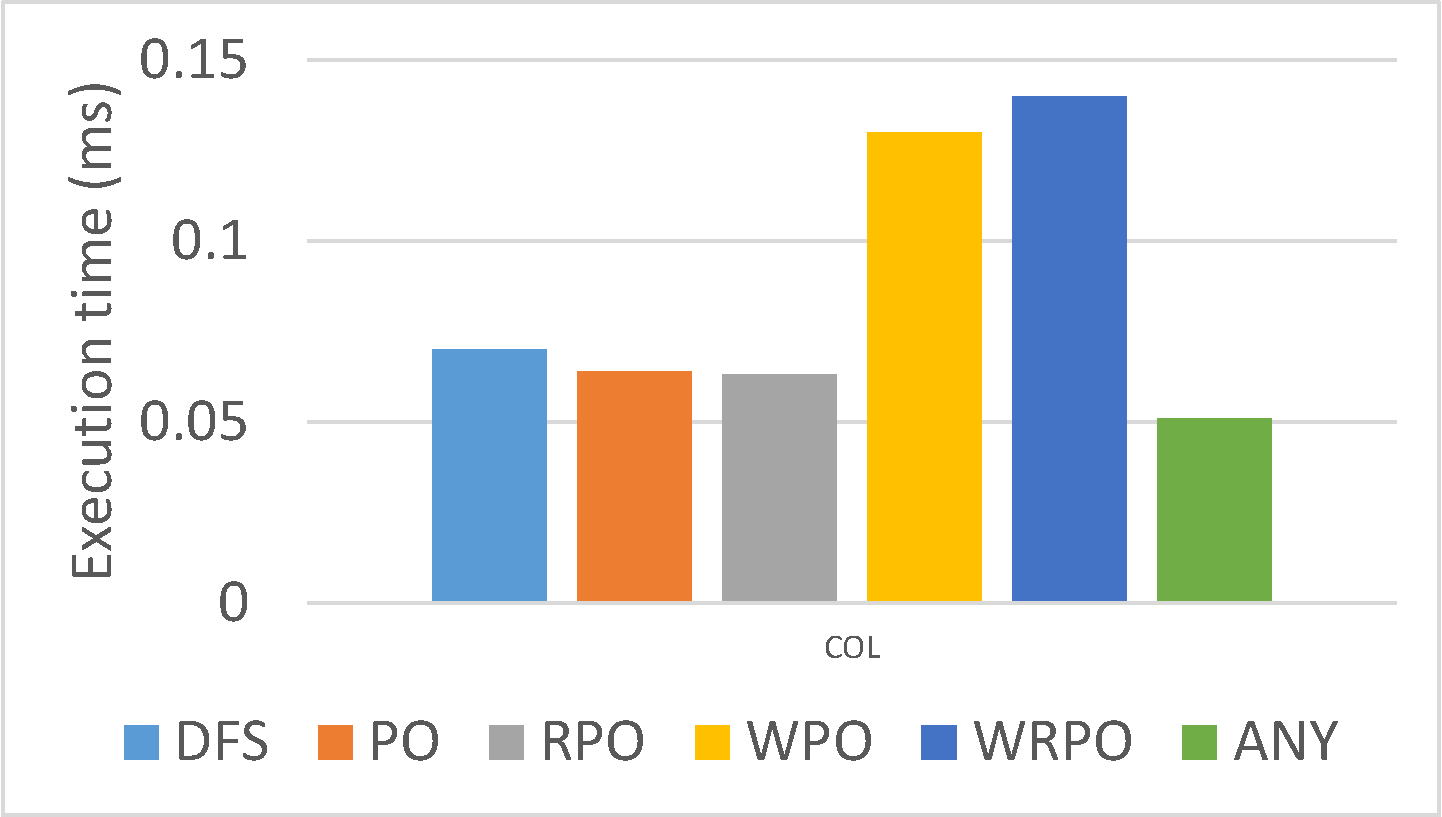
\includegraphics[width=.5\linewidth]{figures/motivation-a-col}
}
\caption{Running times (ms) of the three analyses on graph A using different traversal strategies.}
\label{fig:example-a-graph}
\end{figure*}

{\bf Motivation and Key Observations.\ }
To motivate, consider a software engineering task that infers the temporal 
specifications between pairs of API method calls, i.e., a call to $a$ must be 
followed by a call to $b$ by ~\cite{engler-sosp2001,ramanathan-icse2007,weimer-tacas2005,yang-icse2006}. 
A data-driven approach for inference is to look for pairs of API calls that frequently go in pairs in 
the same order at API call sites in the client methods' code. Such an 
approach contains (at least) three source code analyses on the control flow graph 
(CFG) of each client method: 
%
1) identifying references of the API classes and call sites of the API 
methods which can be done using \emph{reaching definition} analysis(~\cite{programanalysis}); 
%
2) identifying the pairs of API calls ($a$, $b$) where $b$ follows $a$ in the 
client code which can be done using \emph{post-dominator} analysis(~\cite{compilers}); and 
%
3) collecting pairs of temporal API calls by traversing all nodes in the 
CFG--let us call this \emph{collector} analysis. 
%
These analyses need to be run on a large number of client methods to 
produce temporal specifications with high confidence.

Implementing each of these analyses involves traversing the CFG 
of each client method. The traversal strategy could be chosen from a 
set of standard strategies e.g depth-first search (DFS), post-order 
(PO), reverse post-order (RPO), worklist with post-ordering (WPO), 
worklist with reverse post-ordering (WRPO) and any order (ANY).
In ANY order traversal strategy, nodes can
be visited in any order. In post-order traversal, the successors of
any node are visited before visiting the node, while in reverse post-order traversal, the
predecessors of any node are visited before visiting the node. In Worklist with Post-Order and Worklist with reverse post-order, the nodes are visited in the order they appear in the worklist. A worklist is a
data structure used to keep track of nodes to be visited. In WPO, worklist is
initialized with post-ordering of nodes, while in WRPO, The
worklist is initialized with nodes in the reverse post-order.

Figure \ref{fig:example-a-graph} shows the performance of each of these three 
analyses when using standard traversal strategies.
These runs are analyzing the CFG of a method in the DaCapo 
benchmark(~\cite{blackburn2006dacapo}). 
Actual implementation of this method is not important, but it suffices
to know that the CFG, which we shall refer to as Graph A, has 50 nodes
and has branches but no loops. Figure \ref{fig:example-a-graph} shows
that, for graph A, the WRPO performs better than other strategies for
the reaching definition analysis while the WPO outperforms the others
for the post-dominator analysis and the ANY traversal works best for
the collector analysis.

{\bf No Traversal Strategy Fits All.\ } The performance results are
somewhat expected, but require understanding the subtleties of the
analyses. Reaching definition analysis is a forward data-flow analysis
where the output at each node in the graph is dependent on the outputs
of their predecessor nodes.
So, DFS, RPO and WRPO by nature are the most suitable.
However, worklist is the most efficient strategy here because it
visits only the nodes that are yet to reach fixpoint unlike other
strategies that also visit notes that have already reached fixpoint.
Post-dominator analysis, on the other hand, is a backward analysis
meaning that the output at each node in the graph is dependent on the
outputs of their successor nodes. Therefore, the worklist with
post-ordering is the most efficient traversal.
For the collector analysis, any order traversal works better than
other traversal strategies for graph A. This is because for this
analysis the output at each node is not dependent on the output of any
other nodes and hence it is independent of the order of nodes visited.
The any order traversal strategy does not have the overhead of
visiting the nodes in any particular order like DFS, PO, RPO nor the
overhead to maintain the worklist. Therefore any order traversal
performs better than other traversal strategies.

{\bf Properties of Input Graph Determine Strategy.\ }
For the illustrative example discussed above, DFS and RPO were worse
than WRPO for the reaching definition analysis and PO was worse than
WPO for post-dominator because they require one extra iteration of
analysis to be performed and realize that fixpoint has been reached.
However, since graph A does not have any loops, if the graph A's nodes
are visited in such a way that each node is visited after its
predecessors for reaching definition analysis and after its successors
for post-dominator analysis, then the additional iteration is actually
redundant. Given that graph A has no loops, one could optimize RPS or
PO to bypass the extra iteration and fixpoint checking. Thus, the
optimized RPS or PO would run the same number of iterations as the
respective worklist-based ones and finish faster than them because the
overhead of maintaining the list is eliminated.

\begin{figure}
\centering
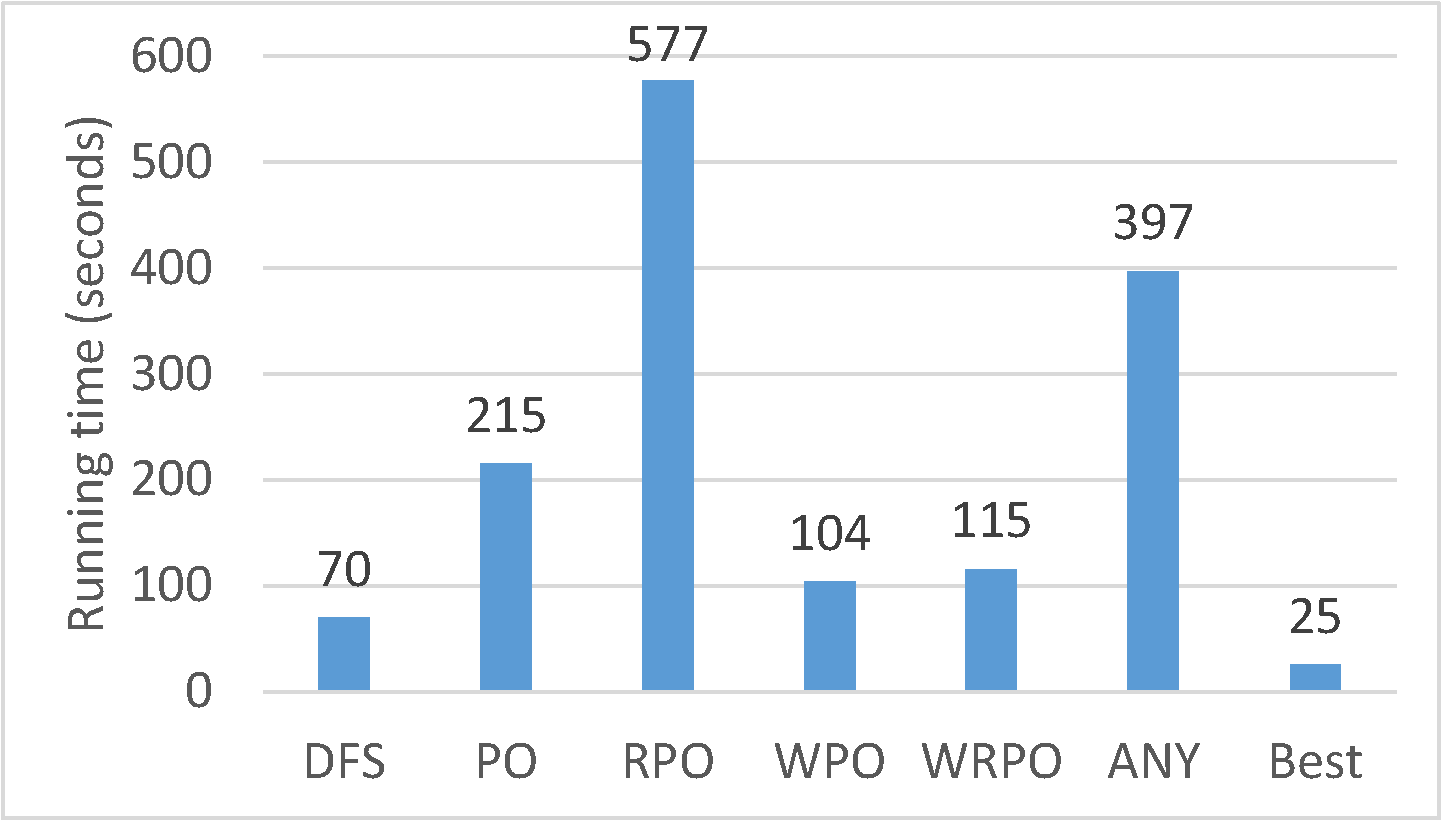
\includegraphics[width=.6\textwidth]{figures/motivation-sum.pdf}
\caption{Running times of three analyses using different traversal strategies on a large codebase.}
\label{fig:motive}
\end{figure}

The potential gains of selecting a suitable traversal strategy can be 
significant.
To illustrate, consider \figref{fig:motive} that shows the performance of 
our entire illustrative example (inferring temporal specifications) on a 
large corpus of 287,000 CFGs extracted from the DaCapo
benchmark dataset(~\cite{blackburn2006dacapo}).
\figref{fig:motive} shows the 
bar chart for the total running times of the three analyses. The \textbf{Best}
 strategy is an ideal one where we can always choose the most efficient with 
all necessary optimizations. The bar chart confirms that fixing a traversal 
strategies for running different analyses on different types of graphs is not 
efficient. Selecting and optimizing traversal strategy for each analysis on 
each graph is desirable. Such a strategy could reduce the running time on a 
large dataset from 64\% (against DFS) to 96\% (against RPO).

Our approach relies on our observations that a suitable traversal strategy is
dependent on both the source code analyses and input graphs' properties.
The former are static properties and the latter are runtime properties.
More importantly, depending on the properties of analyses and graphs, existing
traversals could be optimized to improve their performance.  
We have evaluated our technique using a set of 21 source code analysis that
includes control and data-flow analysis, and analysis to find bugs. The
evaluation is performed on two datasets: a dataset containing well-maintained
projects from DaCapo benchmark (contains a total of 287K graphs), and a
ultra-large dataset containing more than 380K projects from GitHub (contains a
total of 162M graphs). Our evaluation shows that our technique successfully selected
the most time-efficient traversal strategy for 99.99\%--100\% of the time and
using the selected traversal strategy and optimizing it, the running times of a
representative collection of source code analysis in our evaluation
were considerably reduced by 1\%-28\% (13 minutes to 72 minutes in absolute time) when compared against the best performing traversal strategy.
The overhead imposed by our approach is negligible (less than 0.2\% of the total 
running time for a large dataset and less than 0.01\% for an ultra-large dataset). 

The rest of the thesis is organized as follows. Chapter 2 lists the contribution of our work. Chapter 3 gives a background of many ideas that this thesis builds upon, such as Graph and its traversal, various traversal strategies, Program analysis, Control and data flow analysis. Chapter 4.1 describes our system For expressing source code analysis as traversals, while Chapter 4.2 presents the factors that influence the selection of the optimal traversal strategy for any given traversal. Chapter 4.3 lists all the candidate traversal strategies while Chapter 4.4 describes our decision tree to select traversal strategy and also presents an example analysis and graph and walks through the decision tree. Chapter 5 gives the implementation detail on how we extended Boa language to have hybrid capability. Chapter 6 presents our experimental setup and the dataset used. Chapter 7 provides the evaluation and the anlaysis that we did on running time comparison between hybrid and various other strategies. Chapter 8 presents the correctness of analysis using Hybrid approach. Chapter 9 presents the Hybrid's traversal strategy prediction precision. Chapter 10 analyses our decision tree's distribution while Chapter 11 analyses the importance of our traversal optimization. Chapter 12 discusses the two case studies that we implemented using our formalism for source code analysis and their results. Chapter 13 discusses about the threat to validity while Chapter 14 discusses related work. Chapter 15 concludes and gives some possible ideas for future work.